%%%%%%%%%%%%%%%%%%%%%%%%%%%%%%%%%%%%%%%%%%%%%%%%%%%%%%%%%%%%%%%%%%%%%%%%%%%%%%%
%  Laboratorio 4 - Filtros adaptativos LMS en MCXN947
%  Estructura de carpetas (igual que en los TP anteriores):
%     main.tex
%     informe-fcefyn.sty      -> copia de documentacion/TP3/
%     img/                    -> logos, figuras simuladas (las genera
%                                TP4/tools/host_sim/figuras_informe.py)
%     img/placa/              -> capturas tomadas en el laboratorio
%     src/tablas_sim.tex      -> tablas de la simulación (también generadas)
%
%  Capturas del laboratorio que usa este documento (las que falten aparecen
%  como un recuadro rojo con el nombre esperado):
%     img/placa/p1_e1_random_mse.png   tp4_experimentos.m, sección E1
%     img/placa/p1_e2_const_coef.png   tp4_experimentos.m, sección E2
%     img/placa/terminal_p1.png        terminal serie durante una corrida
%     img/placa/osc_d.png              osciloscopio, DAC = d (O0)
%     img/placa/osc_e.png              osciloscopio, DAC = e (O1)
%     img/placa/osc_convergencia.png   DAC = e, disparo en TRIG, SW2
%     img/placa/p2_e6_mu_red.png       tp4_experimentos.m, sección E6
%
%  El Anexo incluye los fuentes de ../../TP4/source y ../../TP4/matlab, con la
%  ruta relativa a esta carpeta (si se compila fuera del repositorio aparece
%  una marca roja en su lugar).
%
%  Todo lo que aparece entre corchetes rojos (\completar{...}) es contenido
%  que falta llenar. Para la entrega, descomentar \entregafinal.
%%%%%%%%%%%%%%%%%%%%%%%%%%%%%%%%%%%%%%%%%%%%%%%%%%%%%%%%%%%%%%%%%%%%%%%%%%%%%%%
\documentclass[11pt,a4paper]{article}
\usepackage{informe-fcefyn}
\usepackage{bm}

% \entregafinal

% ------------------------- Datos de la caratula ------------------------------
\materia{Procesamiento Digital de Señales}
\carrera{Ingeniería en Computación}
\subtitulo{Laboratorio 4}
\tema{Filtros adaptativos LMS en MCXN947}
\plataforma{FRDM-MCXN947 \textperiodcentered{} MCUXpresso IDE \textperiodcentered{} CMSIS-DSP \textperiodcentered{} MATLAB}
\autor{Costamagna, Matias Javier}{44.512.437}{matias.costamagna@mi.unc.edu.ar}
\autor{Moreyra, Julián}{45.214.537}{julian.moreyra@mi.unc.edu.ar}
\autor{Rivera, Mariano}{45.432.921}{luismarianorivera.25@mi.unc.edu.ar}
\autor{Rojas, Facundo Nicolás}{44.629.222}{facundo.rojas.222@mi.unc.edu.ar}
\docentes{Rossi, Roberto Raúl \quad\textperiodcentered\quad Parlanti, Gustavo Fernando \quad\textperiodcentered\quad Molina, Germán Alcides \quad\textperiodcentered\quad Ferreyra, Pablo Alejandro}
\fechaentrega{\today}
\logoizquierdo{img/unc_logo.png}
\logoderecho{img/fcefyn_logo.jpg}

\graphicspath{{img/}}
\newcommand{\Repo}{https://github.com/Mati-Costamagna/procesamiento-digital-de-senales}

% Tablas generadas por la simulación (TP4/tools/host_sim/figuras_informe.py)
% Generado por TP4/tools/host_sim/figuras_informe.py
\newcommand{\TablaPunoSim}{%
\begin{tabular}{llrrrrrl}
\toprule
Entrada & Alg. & $A$ & $\mu$ & $\mu_{max}$ & $\tau$ teó. & MSE final & Estado \\
\midrule
random & CMSIS\_LMS & 1 & 0{,}002 & 0{,}2 & 750 & 5{,}89e-11 & ok \\
random & CMSIS\_LMS & 1 & 0{,}01 & 0{,}2 & 150 & 1{,}15e-12 & ok \\
random & CMSIS\_LMS & 1 & 0{,}05 & 0{,}2 & 30 & 3{,}04e-14 & ok \\
random & CMSIS\_LMS & 1 & 0{,}1 & 0{,}2 & 15 & 6{,}01e-14 & ok \\
random & CMSIS\_LMS & 1 & 0{,}19 & 0{,}2 & 7{,}89 & 1{,}64e-12 & ok \\
random & CMSIS\_LMS & 1 & 0{,}21 & 0{,}2 & 7{,}14 & 1{,}24e+12 & diverge \\
const & CMSIS\_LMS & 1 & 0{,}002 & 0{,}0667 & 8{,}33 & 3{,}20e-14 & ok \\
const & CMSIS\_LMS & 1 & 0{,}01 & 0{,}0667 & 1{,}67 & 0{,}00e+00 & ok \\
const & CMSIS\_LMS & 1 & 0{,}05 & 0{,}0667 & 0{,}333 & 3{,}55e-15 & ok \\
const & CMSIS\_LMS & 1 & 0{,}06 & 0{,}0667 & 0{,}278 & 0{,}00e+00 & ok \\
const & CMSIS\_LMS & 1 & 0{,}07 & 0{,}0667 & 0{,}238 & 4{,}45e+15 & diverge \\
pot & CMSIS\_LMS & 0{,}5 & 0{,}01 & 0{,}8 & 600 & 6{,}03e-12 & ok \\
pot & CMSIS\_LMS & 1 & 0{,}01 & 0{,}2 & 150 & 1{,}15e-12 & ok \\
pot & CMSIS\_LMS & 2 & 0{,}01 & 0{,}05 & 37{,}5 & 1{,}66e-13 & ok \\
pot & CMSIS\_LMS & 5 & 0{,}01 & 0{,}008 & 6 & 6{,}66e+12 & diverge \\
pot & CMSIS\_NLMS & 0{,}5 & 0{,}3 & 2 & 50 & 8{,}58e-15 & ok \\
pot & CMSIS\_NLMS & 1 & 0{,}3 & 2 & 50 & 4{,}07e-14 & ok \\
pot & CMSIS\_NLMS & 2 & 0{,}3 & 2 & 50 & 1{,}36e-13 & ok \\
pot & CMSIS\_NLMS & 5 & 0{,}3 & 2 & 50 & 1{,}22e-12 & ok \\
\bottomrule
\end{tabular}}

\newcommand{\TablaDesajusteSim}{%
\begin{tabular}{rrrrr}
\toprule
$\mu$ & $M$ teórico & MSE teórico & MSE medido & $M$ medido \\
\midrule
0{,}002 & 0{,}010 & 1{,}010e-04 & 1{,}043e-04 & 0{,}043 \\
0{,}01 & 0{,}053 & 1{,}053e-04 & 1{,}088e-04 & 0{,}088 \\
0{,}05 & 0{,}333 & 1{,}333e-04 & 1{,}372e-04 & 0{,}372 \\
0{,}1 & 1{,}000 & 2{,}000e-04 & 2{,}076e-04 & 1{,}076 \\
\bottomrule
\end{tabular}}

\newcommand{\TablaCanceladorSim}{%
\begin{tabular}{lrrrr}
\toprule
Topología & $\mu$ & $\tau$ teó. (s) & Reducción (dB) & SNR salida (dB) \\
\midrule
ruido & 0{,}001 & 1{,}172 & 21{,}2 & 25{,}0 \\
ruido & 0{,}005 & 0{,}234 & 18{,}9 & 22{,}7 \\
ruido & 0{,}02 & 0{,}059 & 13{,}7 & 17{,}5 \\
ruido & 0{,}1 & 0{,}012 & 7{,}5 & 11{,}3 \\
referencia & 0{,}005 & 0{,}234 & 11{,}4 & 15{,}1 \\
referencia & 0{,}02 & 0{,}059 & 7{,}6 & 11{,}3 \\
\bottomrule
\end{tabular}}


% Tipos propios de este trabajo en los listados de código
\lstset{morekeywords=[2]{lms_t,lms_alg_t,p1_cfg_t,p1_io_t,p1_status_t,p2_cfg_t,
  p2_stats_t,p2_out_t,p2_topo_t,prng_t,fir_fijo_t,txt_line_t,
  arm_lms_instance_f32,arm_lms_norm_instance_f32,size_t}}

% \figplaca[ancho]{archivo en img/placa}{descripción}: captura del laboratorio
% dentro de una figura o subfigura; si falta, recuadro rojo como \captura.
\newcommand{\figplaca}[3][0.85\linewidth]{%
  \IfFileExists{img/placa/#2}{\includegraphics[width=#1]{placa/#2}}{%
    \stepcounter{pendientes}%
    \begin{tikzpicture}
      \node[draw=rojoaviso,dashed,thick,rounded corners=3pt,fill=rojoaviso!4,
            minimum width=#1,minimum height=3.2cm,align=center,text width=#1,
            font=\sffamily\small,text=rojoaviso]
        {Captura pendiente: \textbf{#3}\\[3pt] guardar como
         \texttt{img/placa/\detokenize{#2}}};
    \end{tikzpicture}}}

\tikzset{
  blk/.style={draw, thick, rounded corners=2pt, align=center, minimum height=1cm, fill=blue!4},
  sum/.style={draw, thick, circle, inner sep=0pt, minimum size=5mm},
  arr/.style={-{Latex[length=2.2mm]}, thick},
}

\begin{document}

\caratula
\setcounter{tocdepth}{2}
\tableofcontents
\newpage

% ===========================================================================
\section{Introducción}

\begin{consigna}[Laboratorio 4 \textemdash{} Filtros adaptativos]
\textbf{Objetivo.} Verificar el funcionamiento de los sistemas adaptativos e
implementarlos en los DSP de la familia Cortex M4.

\textbf{Parte 1: análisis de un proceso adaptativo.} Realizar un programa en C
que muestre el proceso adaptativo de un filtro transversal de 30 coeficientes,
utilizando el algoritmo LMS y estudiando el mismo con diferentes valores de la
constante de velocidad de adaptación ($\mu$), en el esquema de identificación
de planta. Simular una planta de entrada única con una respuesta al impulso de
30 muestras con valores arbitrarios fijos; calcular el MSE promediándolo cada
100 muestras y mostrar en ese momento la diferencia entre los coeficientes de
la planta y los del filtro adaptativo; usar como entrada una señal
pseudorandom y repetir con una entrada constante. Analizar la influencia de
$\mu$ y de la potencia de entrada.

\textbf{Parte 2: análisis de la influencia del ruido.} Utilizar el mismo FIR de
30 coeficientes para correlacionar la señal random (ruido) con la entrada de
referencia del procesador adaptativo. Ingresar a la placa una senoidal y
sumarle el ruido. Demostrar que el procesador adaptativo converge al filtro
óptimo que cancela el ruido de la señal+ruido y mostrar la señal con un
osciloscopio.
\end{consigna}

La cátedra propone la FRDM-K64F (Cortex-M4); el trabajo se hizo en la
FRDM-MCXN947, cuyo núcleo Cortex-M33 tiene la misma FPU de simple precisión y
las mismas instrucciones DSP, y corre la misma biblioteca CMSIS-DSP.

Todo el código está en la carpeta \archivo{TP4/} del repositorio
\begin{center}\url{\Repo}\end{center}
Ahí están el firmware en \texttt{TP4/source}, los
scripts de MATLAB en \texttt{TP4/matlab} y una simulación en la PC que corre exactamente el
mismo código C en \texttt{TP4/tools/host\_sim}.

% ===========================================================================
\section{Marco teórico}

\subsection{Combinador lineal adaptativo y filtro transversal}
Con una entrada única, el vector de entrada son las últimas $L$ muestras,
$\mathbf{X}_n = [x_n, \dots, x_{n-L+1}]^T$, y la salida es
\begin{equation}
  y_n = \mathbf{W}^T\mathbf{X}_n = \sum_{k=0}^{L-1} w_k\, x_{n-k},
  \qquad e_n = d_n - y_n .
\end{equation}
Si las señales son estacionarias, el error cuadrático medio es una función cuadrática de los
pesos,
\begin{equation}
  \xi = E[e_n^2] = E[d_n^2] - 2\mathbf{P}^T\mathbf{W} + \mathbf{W}^T\mathbf{R}\mathbf{W},
  \qquad \mathbf{R} = E[\mathbf{X}_n\mathbf{X}_n^T],\quad \mathbf{P} = E[d_n\mathbf{X}_n],
\end{equation}
con un único mínimo en el vector de Wiener $\mathbf{W}^* = \mathbf{R}^{-1}\mathbf{P}$, donde
$\xi_{min} = E[d_n^2] - \mathbf{P}^T\mathbf{W}^*$.

\subsection{Máxima pendiente y LMS}
El método de máxima pendiente itera en contra del gradiente,
$\mathbf{W}_{k+1} = \mathbf{W}_k - \mu_{t}\nabla_k$. Trasladando y rotando los ejes a los
vectores propios de $\mathbf{R}$, cada modo $p$ evoluciona en forma independiente como
$(1-2\mu_t\lambda_p)^k$, así que converge si $0 < \mu_t < 1/\lambda_{max}$. Como los autovalores
no se conocen, se usa la cota más segura $0<\mu_t<1/\mathrm{tr}(\mathbf{R})$, con
$\mathrm{tr}(\mathbf{R}) = L\,P_x$ para un filtro transversal ($P_x = E[x_n^2]$).

El LMS reemplaza el gradiente por su estimación instantánea $\hat\nabla_k = -2e_k\mathbf{X}_k$:
\begin{equation}
  \mathbf{W}_{k+1} = \mathbf{W}_k + 2\mu_t\, e_k\mathbf{X}_k .
\end{equation}
No necesita calcular $\mathbf{R}$ ni sus autovalores, ni esperar a juntar muestras: adapta en cada
muestra. En valor medio sigue la misma trayectoria que máxima pendiente, y una vez convergido
queda ``ruido de gradiente'' alrededor de $\mathbf{W}^*$.

\paragraph{Convención usada en el código.} CMSIS-DSP (y la rutina \texttt{LMSfir} de la clase)
escriben la actualización como $w_k \leftarrow w_k + \mu\, e_n\, x_{n-k}$, es decir
$\mu = 2\mu_t$. En todo el informe se usa el $\mu$ de CMSIS, con lo que las fórmulas quedan:
\begin{align}
  &\text{convergencia:} && 0 < \mu < \frac{2}{\lambda_{max}} \;\Rightarrow\; 0<\mu<\frac{2}{L\,P_x}
  \quad\text{(cota segura)}\label{eq:mumax}\\
  &\text{constante de tiempo del MSE:} && \tau_{mse,p} \approx \frac{1}{2\mu\lambda_p}\ \text{muestras}\label{eq:tau}\\
  &\text{desajuste:} && M = \frac{\xi_{exceso}}{\xi_{min}} \approx \frac{\mu\,\mathrm{tr}(\mathbf{R})/2}{1-\mu\,\mathrm{tr}(\mathbf{R})/2}
  \approx \frac{\mu}{2} L P_x \label{eq:M}
\end{align}

\subsection{LMS normalizado}
En el NLMS (\texttt{arm\_lms\_norm\_f32}) el paso se divide por la energía de la entrada en la
ventana del filtro, $E_n = \sum_{k=0}^{L-1}x_{n-k}^2 \approx L P_x$:
$w_k \leftarrow w_k + \mu\, e_n x_{n-k}/E_n$. El paso efectivo es $\mu/(LP_x)$, así que la
condición $0<\mu<2$ y la velocidad de convergencia ya no dependen de la potencia de la entrada.

\subsection{Esquemas usados}
\textbf{Identificación de planta:} la entrada $x$ excita a la planta $P(z)$ y al filtro
adaptativo; la salida de la planta es la señal deseada $d$. Si la entrada es suficientemente
rica, $\mathbf{W}^*$ es la respuesta al impulso de la planta.
\textbf{Cancelador de interferencia:} $d = s + n'$, donde la señal útil $s$ está contaminada con
un ruido $n'$, y el filtro recibe una referencia $x$ distinta pero correlacionada con $n'$ y no
con $s$. El filtro estima $n'$ a partir de $x$ y el error $e = s + n' - y$ tiende a $s$.

% ===========================================================================
\section{Materiales y conexionado}
\begin{table}[H]
\centering
\caption{Equipamiento.}
\small
\begin{tabular}{ll}
\toprule
Placa & NXP FRDM-MCXN947 (MCXN947, Cortex-M33 a 150 MHz, FPU y DSP) \\
Entorno & MCUXpresso IDE v11.10.0, SDK FRDM-MCXN947, CMSIS-DSP \\
PC & MATLAB (R2019b o posterior) y terminal serie a 115200 baud \\
Generador de funciones & \completar{modelo} \\
Osciloscopio & \completar{modelo} \\
\bottomrule
\end{tabular}
\end{table}

\begin{table}[H]
\centering
\caption{Conexiones de la Parte 2 (la Parte 1 sólo usa el USB).}
\label{tab:pines}
\footnotesize
\begin{tabular}{llll}
\toprule
Señal & Pin MCU & Conector & Uso \\
\midrule
Entrada analógica (ADC0, canal A2) & P4\_23 & J8 pin 28 & senoidal del generador \\
Salida DAC0 & P4\_2 & J1 pin 4 & canal 2 del osciloscopio \\
TRIG (pulso al reiniciar $\mathbf{W}$) & P1\_23 & J1 pin 8 & disparo externo \\
PROC (en alto mientras procesa) & P4\_0 & J2 pin 18 & tiempo de cómputo \\
GND & -- & cualquier GND & masa común \\
Puerto serie (LPUART4) & P1\_8 / P1\_9 & USB J17 (MCU-Link) & VCOM \\
\bottomrule
\end{tabular}
\end{table}

El ADC mide de 0 a 3,3~V, así que la senoidal se monta sobre 1,65~V de continua (1~Vpp, salida
del generador en High-Z). El firmware estima y resta esa continua con un filtro de seguimiento
lento ($\alpha = 2^{-12}$), y el DAC saca la señal elegida centrada en 1,65~V.

% ===========================================================================
\section{Diseño de la aplicación}

\subsection{Organización del firmware}
Las dos partes van en un único programa; se pasa de una a otra con una pulsación larga de SW3 o
con los comandos \texttt{1} y \texttt{2} por el puerto serie. El procesamiento está separado del
hardware: \texttt{parte1.c} y \texttt{parte2.c} sólo reciben y devuelven números, y
\texttt{main.c} hace de ``placa'' (teclas, UART, ADC, DAC, timer). Así el mismo código se compila
también en la PC (\texttt{TP4/tools/host\_sim}), lo que permitió verificar los algoritmos y
generar las figuras simuladas de este informe antes de ir al laboratorio.

\begin{table}[H]
\centering
\caption{Módulos del firmware.}
\begin{tabular}{p{3.2cm}p{11.3cm}}
\toprule
\texttt{lms.c/.h} & Filtro adaptativo con tres implementaciones intercambiables: la rutina
\texttt{LMSfir} de la clase, \texttt{arm\_lms\_f32} y \texttt{arm\_lms\_norm\_f32}. \\
\texttt{parte1.c/.h} & Identificación de planta: entrada, planta, LMS, MSE cada 100 muestras. \\
\texttt{parte2.c/.h} & Cancelador: ruido, correlador, LMS, estadísticas por bloque. \\
\texttt{coefs.c/.h} & Coeficientes fijos de la planta y del correlador. \\
\texttt{fir\_fijo.h} & FIR de coeficientes fijos con buffer circular. \\
\texttt{prng.h} & Generador pseudoaleatorio xorshift32 (uniforme en $[-1,1)$). \\
\texttt{txt\_out.c/.h} & Arma las líneas CSV con floats sin depender de \texttt{printf}. \\
\texttt{main.c} & Periféricos, teclas, comandos, ISR de muestreo. \\
\texttt{app\_config.h} & Todos los parámetros ajustables. \\
\bottomrule
\end{tabular}
\end{table}

\paragraph{Generador pseudoaleatorio.} Se usa un xorshift32 propio en lugar de \texttt{rand()}
para que la secuencia sea la misma en la placa y en la PC, y para repetir un experimento con
la misma entrada cambiando sólo $\mu$ (todas las corridas de un barrido usan la semilla 1). Con
24 bits de mantisa se obtiene una uniforme en $[-A, A)$, de media nula y $P_x = A^2/3$.

\paragraph{Implementaciones del LMS.} La rutina de la diapositiva ``Implementación en DSP'' se
pasó a \texttt{lms\_clase\_step()}: desplaza la línea de retardo, calcula $y$ y adapta. La única
diferencia es que el error $d-y$ se calcula una vez, con la salida completa de la muestra actual,
antes de adaptar; en la versión de la diapositiva que funde los tres lazos, el $(d-y)$ usa la $y$
parcial que se va acumulando. Las funciones de CMSIS se llaman con \texttt{blockSize = 1}
(muestra a muestra) y guardan los coeficientes en orden invertido en el tiempo, por lo que
\texttt{lms\_get\_w()} los da vuelta para compararlos con la planta.

\subsection{Parte 1: identificación de planta}
\begin{figure}[H]
\centering
\begin{tikzpicture}[node distance=1.2cm and 1.5cm]
  \node[blk] (rnd) {Entrada\\random / constante};
  \node[blk, right=1.6cm of rnd] (pl) {PLANTA $P(z)$\\FIR 30 coef. fijos};
  \node[sum, right=1.1cm of pl] (sv) {$+$};
  \node[above=0.6cm of sv] (v) {$v_n$ (opcional)};
  \node[sum, right=1.4cm of sv] (s) {$\Sigma$};
  \node[blk, below=1.0cm of pl] (af) {FIR ADAPTATIVO $W(z)$\\30 coef. -- LMS};
  \node[right=1.2cm of s] (e) {$e_n$};
  \coordinate[left=0.8cm of pl] (bif);
  \draw[arr] (rnd) -- node[above]{$x_n$} (pl);
  \draw[arr] (bif) |- (af);
  \fill (bif) circle (1.5pt);
  \draw[arr] (pl) -- (sv);
  \draw[arr] (v) -- (sv);
  \draw[arr] (sv) -- node[above]{$d_n$} node[below right, pos=0.85]{\scriptsize $+$} (s);
  \draw[arr] (af) -| node[pos=0.25, above]{$y_n$} node[pos=0.92, right]{\scriptsize $-$} (s);
  \draw[arr] (s) -- (e);
  \draw[arr, dashed] ($(s)+(0.6,0)$) |- ($(af.south)+(0,-0.5)$) -- ($(af.south)+(0,0)$);
  \node[draw, dashed, gray, fit=(rnd)(pl)(af)(s)(v), inner sep=8pt, label={[gray]below left:FRDM-MCXN947}] {};
\end{tikzpicture}
\caption{Esquema de identificación de planta implementado (figura 1 de la consigna). Todo
corre dentro del microcontrolador.}
\label{fig:p1diag}
\end{figure}

La planta tiene una respuesta al impulso de 30 muestras con valores arbitrarios fijos,
$p_k = 0{,}8\,e^{-k/8}\sin(0{,}3\pi(k+1)) + 0{,}05\cos(0{,}9k)$ redondeados a 4 decimales
($\sum p_k^2 = 1{,}979$). Cada experimento procesa $N = 20000$ muestras en bloques de 100. Al
final de cada bloque se envía por el puerto serie:
\begin{itemize}
  \item \texttt{P1M,n,mse,werr2,mse\_dB}: el MSE promedio de las 100 muestras,
  $\frac{1}{100}\sum e_n^2$, y el error de los coeficientes $\|\mathbf{p}-\mathbf{w}\|^2$;
  \item \texttt{P1D,n,d0,...,d29}: la diferencia $p_k - w_k$ de cada uno de los 30 coeficientes.
\end{itemize}
Al principio se manda la configuración (\texttt{P1I}, que incluye $\mu_{max}$ y $\tau$ teóricos)
y la planta (\texttt{P1P}); al final los coeficientes aprendidos (\texttt{P1W}) y los ciclos de
CPU promedio por muestra del LMS medidos con el contador \texttt{DWT->CYCCNT} (\texttt{P1F}). Si
el MSE supera $10^{12}$ la corrida se corta y se informa \texttt{DIVERGE}.

\subsection{Parte 2: cancelador de ruido}
\begin{figure}[H]
\centering
\begin{tikzpicture}
  \node[blk] (gen) at (0,0) {Generador\\senoidal};
  \node[blk] (adc) at (2.3,0) {ADC0\\16 bits};
  \node[blk] (dc) at (4.4,0) {$-$ continua};
  \node[sum] (s1) at (7.2,0) {$+$};
  \node[sum] (s2) at (10.2,0) {$\Sigma$};
  \node[blk] (dac) at (11.7,0) {DAC0};
  \node (osc) at (13.1,0) {Osc.};
  \node[blk] (rnd) at (3.0,-1.8) {random $r_n$};
  \node[blk] (cor) at (7.2,-1.8) {CORRELADOR $C(z)$\\FIR 30 coef. fijos};
  \node[blk] (af) at (6.6,-3.6) {FIR ADAPTATIVO $W(z)$\\30 coef. -- LMS};
  \draw[arr] (gen) -- (adc);
  \draw[arr] (adc) -- (dc);
  \draw[arr] (dc) -- node[above]{$s_n$} (s1);
  \draw[arr] (rnd) -- (cor);
  \draw[arr] (cor) -- node[right]{$n'_n$} (s1);
  \draw[arr] (s1) -- node[above]{$d_n$} node[below left, pos=0.85]{\scriptsize $+$} (s2);
  \draw[arr] (rnd.south) |- node[pos=0.3, left]{$x_n = r_n$} (af.west);
  \draw[arr] (af.east) -| node[pos=0.7, left]{$y_n \approx n'_n$} node[pos=0.93, right]{\scriptsize $-$} (s2);
  \draw[arr] (s2) -- node[above]{$e_n$} (dac);
  \draw[arr] (dac) -- (osc);
  \draw[arr, dashed] (10.9,0) |- ($(af.south)+(0,-0.45)$) -- (af.south);
  \node[draw, dashed, gray, fit=(adc)(dc)(s2)(dac)(rnd)(af), inner sep=9pt,
        label={[gray]below right:FRDM-MCXN947}] {};
\end{tikzpicture}
\caption{Cancelador implementado. El ruido $r_n$ se genera adentro de la placa, pasa por el
correlador y se suma a la senoidal; el filtro adaptativo recibe $r_n$ como referencia. Por el
DAC se puede sacar $d$, $e$, $y$, $s$ o el residuo $e-s$.}
\label{fig:p2diag}
\end{figure}

El CTIMER0 marca $f_s = 8$~kHz y en cada período dispara una conversión del ADC. Toda la
cadena de la figura~\ref{fig:p2diag} corre en la interrupción del ADC, muestra a muestra:
\begin{enumerate}
  \item se convierte la lectura a volts y se resta la continua: $s_n$;
  \item se genera $r_n$ uniforme en $[-0{,}4, 0{,}4]$~V y se filtra con el correlador: $n'_n = C\{r\}_n$;
  \item $d_n = s_n + n'_n$, y el LMS con referencia $x_n = r_n$ da $y_n$ y $e_n = d_n - y_n$;
  \item la señal elegida se escribe en el DAC.
\end{enumerate}

El correlador es $c_k = 0{,}6\cdot 0{,}8^k$, $k = 0\dots29$ (energía $\sum c_k^2 = 1$, así que
el ruido mantiene su potencia: $P_{n'} = P_r = 0{,}4^2/3 = 0{,}0533$~V$^2$). Como $r_n$ es
blanco, $\mathbf{R} = P_r\mathbf{I}$ y $\mathbf{P} = E[d_n\mathbf{X}_n] = P_r\,\mathbf{c}$, de modo que
el filtro óptimo es exactamente $\mathbf{W}^* = \mathbf{c}$: el procesador tiene que
\emph{copiar} al correlador. Con eso $y = n'$ y $e = s$.

Como el ruido se genera en la placa, también se conoce $s_n$ limpia, y se puede medir cuánto
ruido queda a la salida: el residuo $e_n - s_n$. Cada 100 muestras se envía
una línea \texttt{P2M} con la potencia del ruido, la del residuo, la reducción en dB, $\|\mathbf{W}^*-\mathbf{w}\|^2$ y las SNR de entrada y salida. Se usa
$\|\mathbf{W}^*-\mathbf{w}\|^2$ como medida de convergencia al óptimo. SW2 pone los
coeficientes en cero y genera un pulso en TRIG, para disparar el osciloscopio justo cuando el
filtro empieza a aprender.

\paragraph{Ubicación del correlador.} La figura 2 de la consigna dibuja el correlador en la rama
de la referencia: $d = s + r$ y $x' = C\{r\}$. En ese caso el óptimo es $\mathbf{W}^* = C^{-1}$,
que existe y es estable sólo si $C(z)$ es de fase mínima. Se eligió un correlador de fase
mínima (sus ceros están en $|z| = 0{,}8$) y casi igual a $0{,}6/(1-0{,}8z^{-1})$, de modo que
$C^{-1}(z) \approx (1-0{,}8z^{-1})/0{,}6$: un FIR de dos coeficientes, $[1{,}667;\ -1{,}333]$.
Las dos variantes están implementadas (comando \texttt{Q0} / \texttt{Q1}); por defecto se usa
la del correlador en el camino del ruido, que es la del cancelador de interferencia de la teoría.

\subsection{Interfaz}
\begin{table}[H]
\centering
\caption{Teclas y comandos (letra + valor + Enter, desde cualquier terminal o MATLAB).}
\begin{tabular}{lp{11cm}}
\toprule
SW3 largo / \texttt{1}, \texttt{2} & Cambia entre Parte 1 (LED verde) y Parte 2 (LED rojo). \\
SW2 & P1: arranca (o corta) un experimento. P2: reinicia los coeficientes + pulso en TRIG. \\
SW3 corto & P1: siguiente $\mu$ de la lista. P2: cambia la señal del DAC ($d$, $e$, $y$, $s$, residuo). \\
\texttt{U<mu>}, \texttt{G<0|1|2>} & Paso de adaptación; algoritmo (clase, \texttt{arm\_lms\_f32}, NLMS). \\
\texttt{A<amp>} & P1: amplitud de la entrada. P2: amplitud del ruido. \\
\texttt{E<0|1>}, \texttt{V<sv>}, \texttt{S}, \texttt{B} & P1: entrada aleatoria/constante, ruido de medición, arrancar, barrido de $\mu$. \\
\texttt{Q}, \texttt{O}, \texttt{Z}, \texttt{C}, \texttt{T}, \texttt{F} & P2: topología, salida del DAC, reinicio, coeficientes, tiempos, $f_s$. \\
\bottomrule
\end{tabular}
\end{table}

% ===========================================================================
\section{Resultados de la Parte 1}
Las figuras de esta sección se generaron corriendo en la PC el mismo código del firmware
(\texttt{p1\_sim}), con la misma CMSIS-DSP. En la placa se repiten con
\texttt{tp4\_experimentos.m}, que manda los mismos comandos y produce las mismas figuras
(sección~\ref{sec:placa1}).

\subsection{Influencia de $\mu$ con entrada aleatoria}
Con $A = 1$, $P_x = 1/3$ y la cota (\ref{eq:mumax}) da $\mu_{max} = 2/(30\cdot1/3) = 0{,}2$.
Como la entrada es blanca, $\mathbf{R} = P_x\mathbf{I}$: los 30 autovalores son iguales y
(\ref{eq:tau}) da $\tau_{mse} = 1/(2\mu P_x) = 1{,}5/\mu$ muestras.

\begin{figure}[H]
\centering
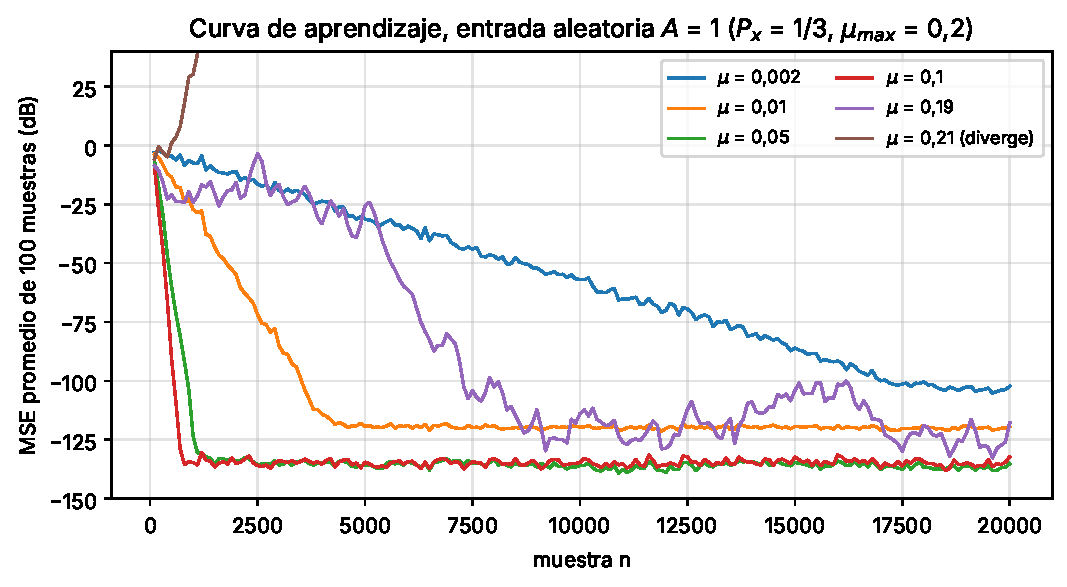
\includegraphics[width=0.9\linewidth]{p1_e1_mse.pdf}
\caption{Curva de aprendizaje (MSE promediado cada 100 muestras) para distintos $\mu$.}
\label{fig:e1mse}
\end{figure}

\begin{itemize}
  \item La pendiente de la curva en dB es $-10\log_{10}(e)/\tau \approx -4{,}34/\tau$ dB por
  muestra. Para $\mu = 0{,}01$ ($\tau = 150$) se esperan 29~dB cada 1000 muestras, y la curva
  baja de $-3$ a $-55$~dB en las primeras 2000: coincide.
  \item Sin ruido de medición $\xi_{min} = 0$, así que el MSE baja hasta el piso de la aritmética
  de punto flotante de simple precisión ($-120$ a $-135$~dB) y los coeficientes llegan
  exactamente a los de la planta (figura~\ref{fig:e1coef}).
  \item Hasta $\mu \approx 0{,}05$--$0{,}1$, aumentar $\mu$ acelera el aprendizaje. Más cerca del
  límite ($\mu = 0{,}19$) el proceso se vuelve errático y más \emph{lento}, y con
  $\mu = 0{,}21 > \mu_{max}$ diverge. La cota $2/\mathrm{tr}(\mathbf{R})$ resultó muy ajustada:
  para el LMS (no para máxima pendiente, que con autovalores iguales admitiría hasta
  $2/P_x = 6$) el límite real de estabilidad en media cuadrática está cerca de
  $2/\mathrm{tr}(\mathbf{R})$, porque el ruido del gradiente crece con $\mu\,\mathrm{tr}(\mathbf{R})$.
\end{itemize}

\begin{figure}[H]
\centering
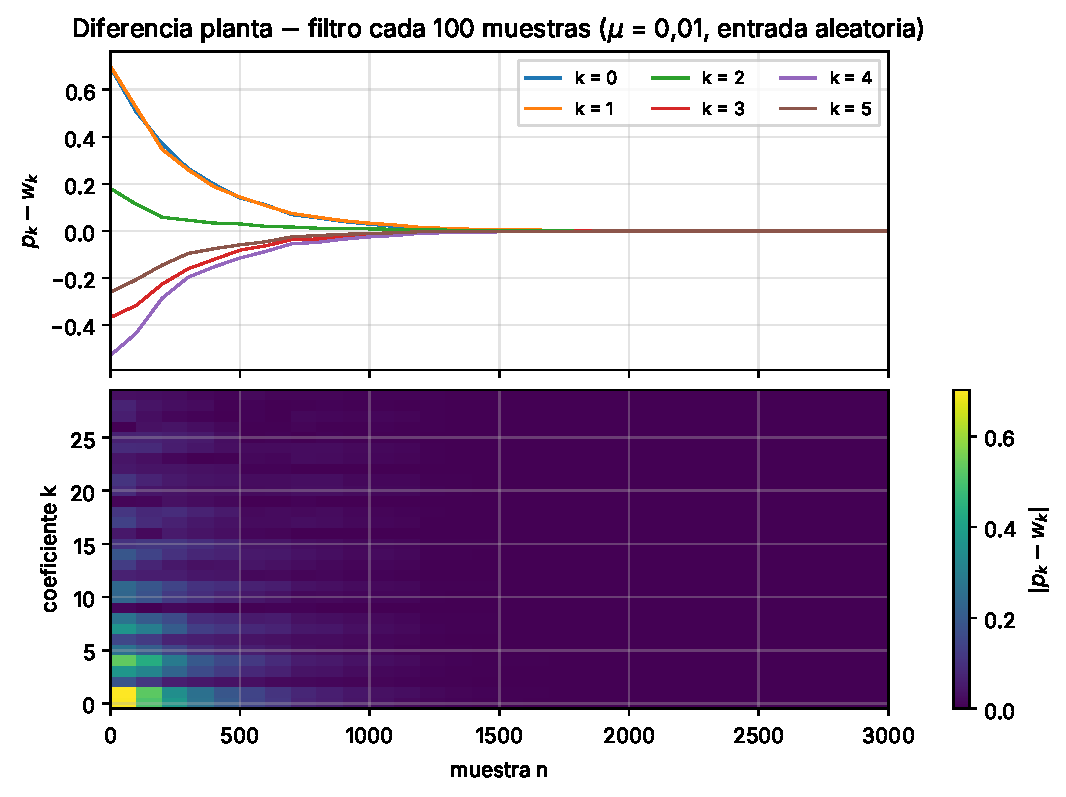
\includegraphics[width=0.9\linewidth]{p1_e1_diff.pdf}
\caption{Diferencia entre los coeficientes de la planta y los del filtro, mostrada cada 100
muestras ($\mu = 0{,}01$). Arriba, los 6 primeros coeficientes; abajo, $|p_k - w_k|$ de los 30.}
\label{fig:e1diff}
\end{figure}

\begin{figure}[H]
\centering
\begin{subfigure}{0.49\linewidth}
  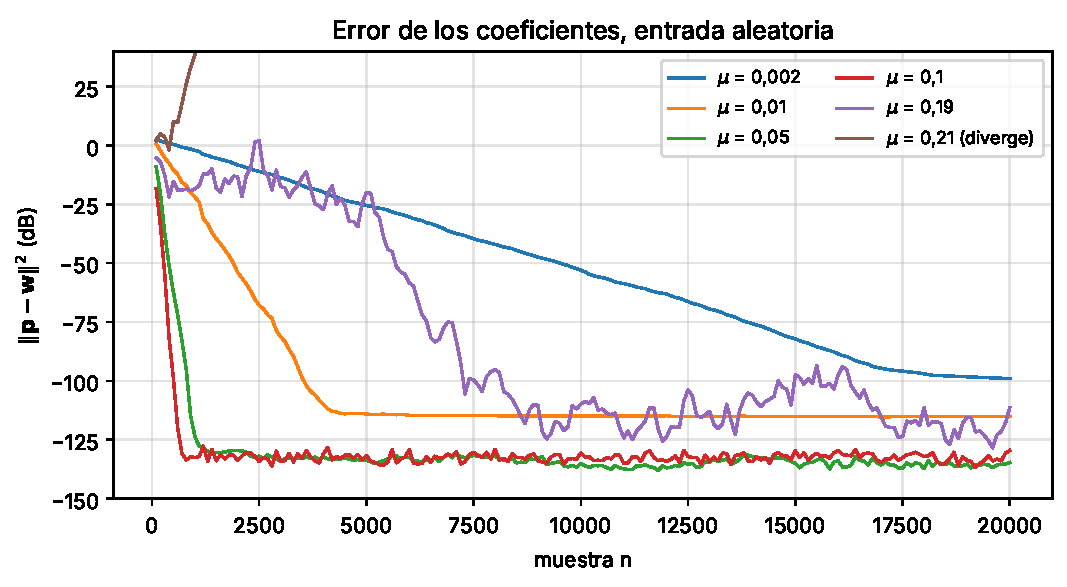
\includegraphics[width=\linewidth]{p1_e1_werr.pdf}
  \caption{$\|\mathbf{p}-\mathbf{w}\|^2$.}
\end{subfigure}
\begin{subfigure}{0.49\linewidth}
  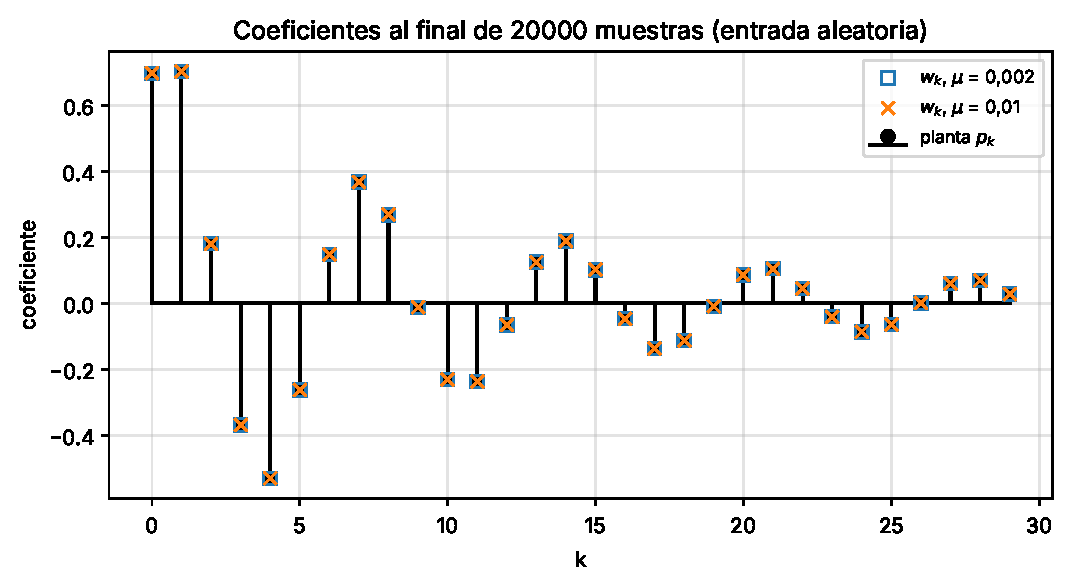
\includegraphics[width=\linewidth]{p1_e1_coef.pdf}
  \caption{Coeficientes finales.}
  \label{fig:e1coef}
\end{subfigure}
\caption{Error de los coeficientes y coeficientes aprendidos con entrada aleatoria.}
\end{figure}

\subsection{Entrada constante}
Con $x_n = A$, $\mathbf{R} = A^2\mathbf{1}\mathbf{1}^T$ tiene un solo autovalor no nulo,
$\lambda = LA^2 = \mathrm{tr}(\mathbf{R})$, con vector propio $\mathbf{1}$, y 29 autovalores
nulos. El MSE sólo ``ve'' la componente de $\mathbf{w}$ en la dirección de $\mathbf{1}$, es
decir, la suma de los coeficientes (la ganancia en continua). En consecuencia:
\begin{itemize}
  \item El MSE converge a cero muy rápido ($\tau = 1/(2\mu L A^2)$, menos de 10 muestras), pero
  sólo porque $\sum w_k = \sum p_k$ (la ganancia de continua): figura~\ref{fig:e2coef}.
  \item Los coeficientes \textbf{no} se identifican: $\|\mathbf{p}-\mathbf{w}\|^2$ queda cerca
  de $\|\mathbf{p}\|^2$. Los modos con $\lambda = 0$ no se adaptan nunca. Es la
  ``solución parcial por falta de excitación apropiada'' de la teoría. (Los primeros
  coeficientes se mueven un poco porque al arrancar la línea de retardo se llena desde cero,
  lo que equivale a un escalón con algo de excitación.)
  \item La cota de estabilidad es la misma fórmula, $\mu < 2/(LA^2) = 0{,}0667$: con
  $\mu = 0{,}07$ diverge. La entrada constante tiene el triple de potencia que la aleatoria de la
  misma amplitud, y por eso diverge con un $\mu$ tres veces menor.
\end{itemize}

\begin{figure}[H]
\centering
\begin{subfigure}{0.49\linewidth}
  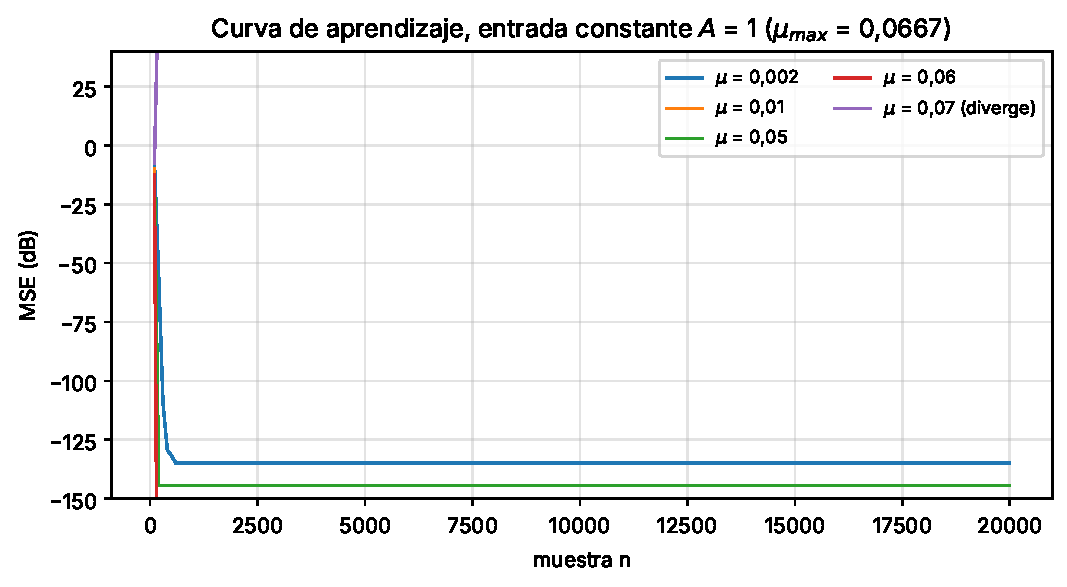
\includegraphics[width=\linewidth]{p1_e2_mse.pdf}
\end{subfigure}
\begin{subfigure}{0.49\linewidth}
  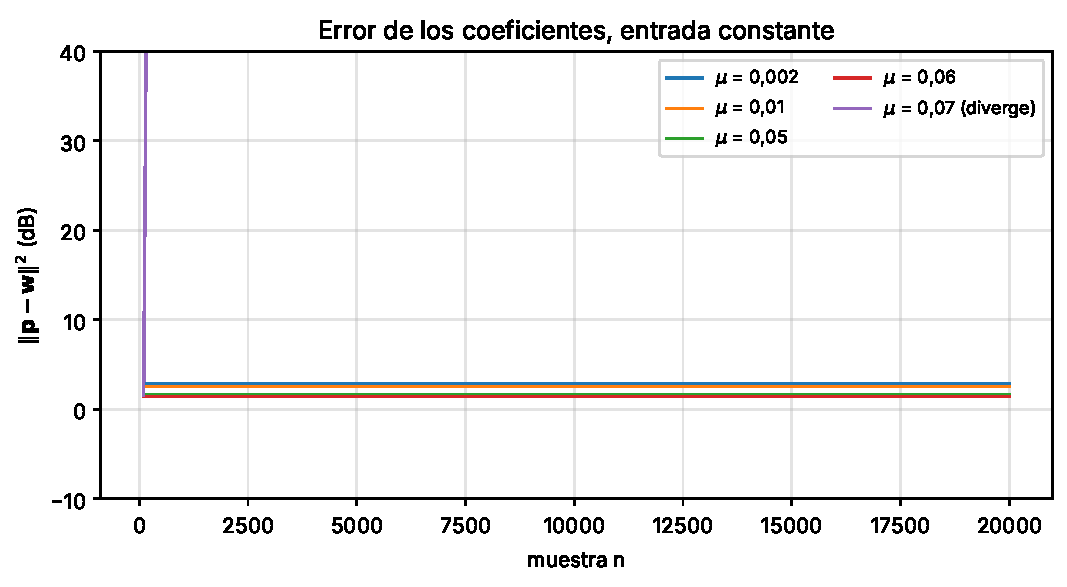
\includegraphics[width=\linewidth]{p1_e2_werr.pdf}
\end{subfigure}
\caption{Entrada constante: el MSE llega al piso numérico pero el error de los coeficientes no baja.}
\end{figure}

\begin{figure}[H]
\centering
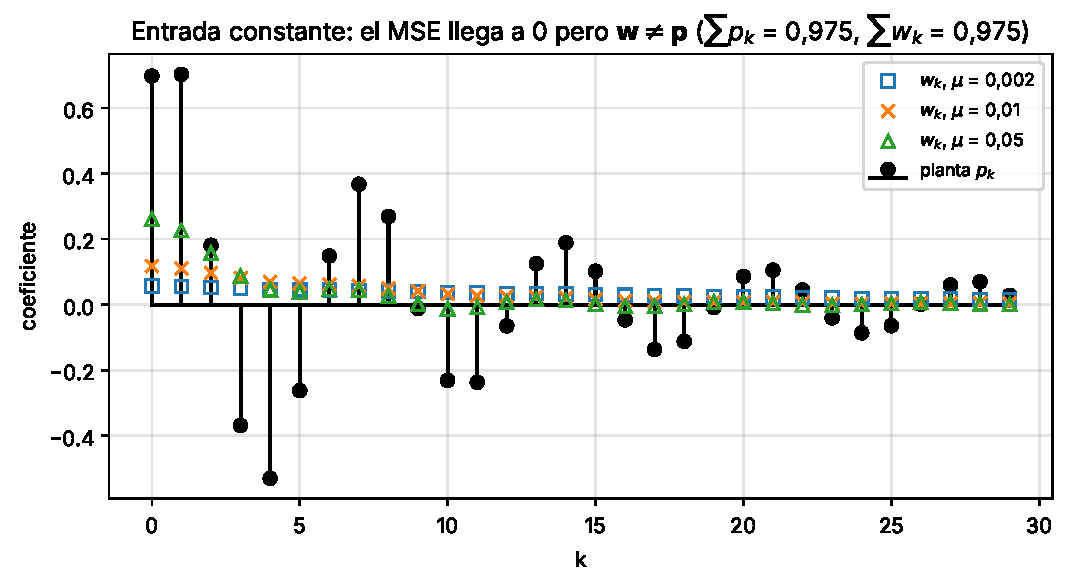
\includegraphics[width=0.85\linewidth]{p1_e2_coef.pdf}
\caption{Con entrada constante el filtro aprende una respuesta distinta de la planta pero con la
misma ganancia de continua.}
\label{fig:e2coef}
\end{figure}

\subsection{Influencia de la potencia de entrada}
Con el LMS, $\mu_{max}$ y $\tau$ dependen de $P_x$: con $\mu = 0{,}01$ fijo, duplicar la amplitud
multiplica $P_x$ por 4, divide $\tau$ por 4 (más rápido) y divide $\mu_{max}$ por 4. Con
$A = 5$, $\mu_{max} = 0{,}008 < 0{,}01$ y el filtro diverge. El NLMS normaliza el paso con la
energía de la entrada: las cuatro curvas son prácticamente iguales
(figura~\ref{fig:e3}). El piso numérico sube con $A$ porque crece la escala de las señales.

\begin{figure}[H]
\centering
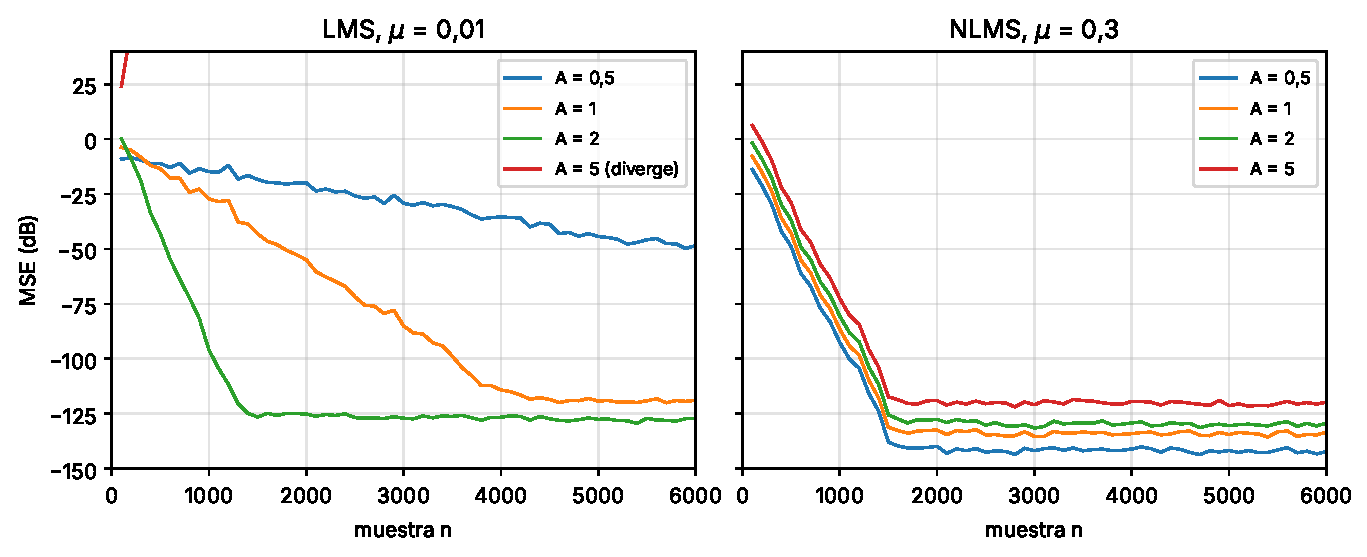
\includegraphics[width=\linewidth]{p1_e3_potencia.pdf}
\caption{Misma planta y mismo $\mu$ con distintas amplitudes de entrada: LMS (izquierda) y NLMS (derecha).}
\label{fig:e3}
\end{figure}

\subsection{Ruido de medición y desajuste}
Si a la salida de la planta se suma un ruido $v_n$ de varianza $\sigma_v^2$ (comando
\texttt{V}), $\xi_{min} = \sigma_v^2$ y el MSE en régimen es $\sigma_v^2(1+M)$. Con
$\sigma_v = 0{,}01$ ($-40$~dB) aparece el compromiso típico: un $\mu$ más grande converge más
rápido pero deja más ruido de gradiente. Los valores medidos en las últimas 5000 muestras siguen
a (\ref{eq:M}) (tabla~\ref{tab:desajuste}); el pequeño exceso es la variabilidad de estimar una
potencia con bloques de 100 muestras.

\begin{figure}[H]
\centering
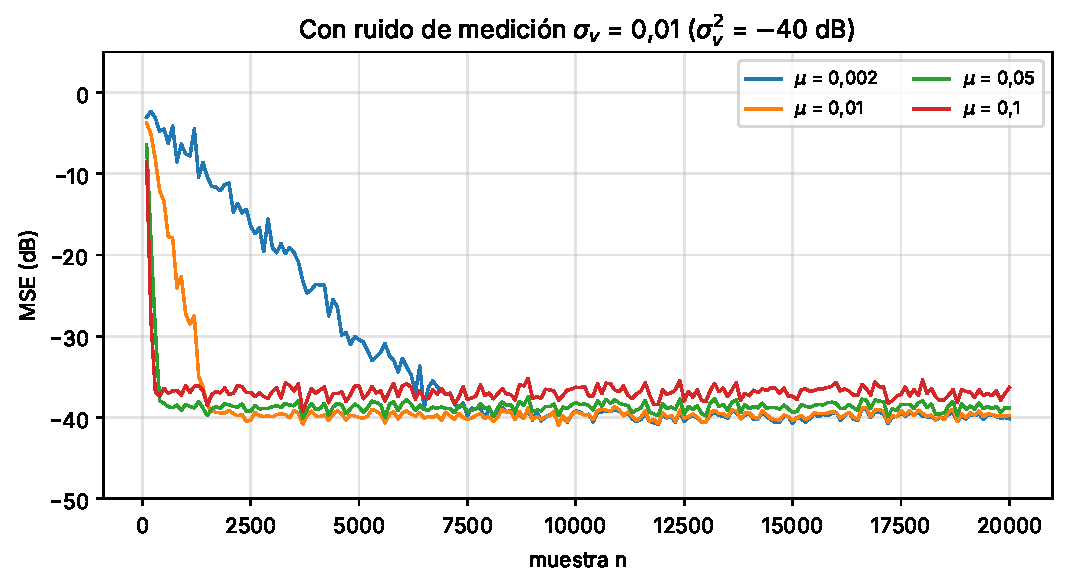
\includegraphics[width=0.85\linewidth]{p1_e5_mse.pdf}
\caption{Curvas de aprendizaje con ruido de medición $\sigma_v = 0{,}01$.}
\end{figure}

\begin{table}[H]
\centering
\caption{Desajuste con $\sigma_v = 0{,}01$, entrada aleatoria $A = 1$ (simulación).}
\label{tab:desajuste}
\TablaDesajusteSim
\end{table}

\subsection{Comparación de implementaciones}
La rutina de la clase y \texttt{arm\_lms\_f32} dan curvas idénticas bit a bit en la simulación
(hacen las mismas operaciones en el mismo orden). El NLMS con $\mu = 0{,}3$ equivale a un LMS con
$\mu = 0{,}3/(LP_x) = 0{,}03$. En la placa se mide el costo de cada una (tabla~\ref{tab:ciclos}).

\begin{figure}[H]
\centering
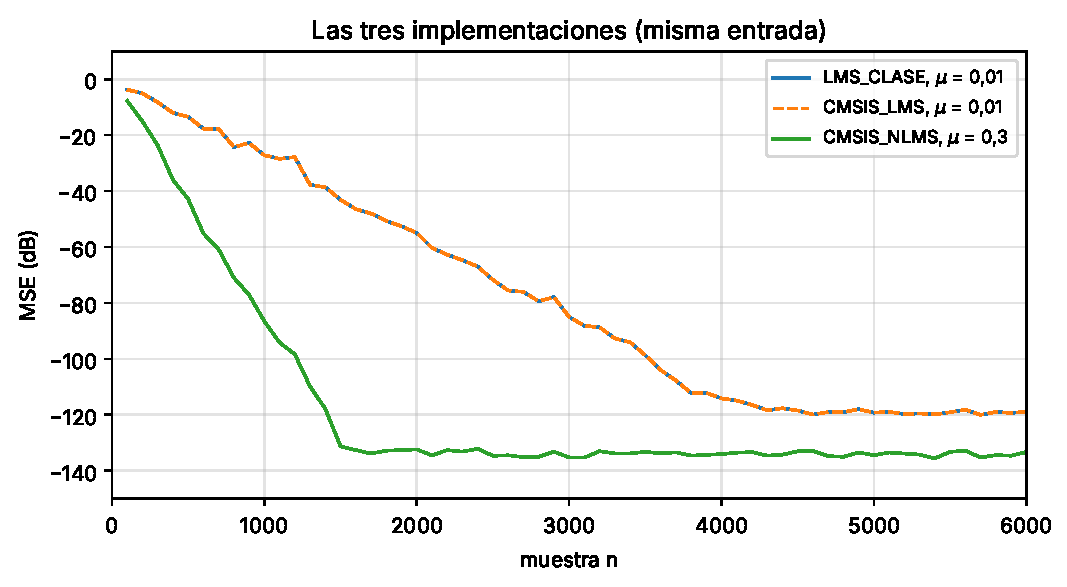
\includegraphics[width=0.8\linewidth]{p1_e4_alg.pdf}
\caption{Las tres implementaciones con la misma entrada.}
\end{figure}

\begin{table}[H]
\centering
\caption{Resumen de las corridas de la Parte 1 (simulación). $\tau$ en muestras.}
\small
\TablaPunoSim
\end{table}

\subsection{Resultados en la placa}\label{sec:placa1}
\begin{figure}[H]
\centering
\figplaca{p1_e1_random_mse.png}{Curva de aprendizaje medida (tp4\_experimentos.m, sección E1)}
\caption{Curva de aprendizaje medida en la FRDM-MCXN947, entrada aleatoria.}
\end{figure}
\begin{figure}[H]
\centering
\figplaca{p1_e2_const_coef.png}{Coeficientes con entrada constante (sección E2)}
\caption{Coeficientes finales medidos con entrada constante.}
\end{figure}
\begin{figure}[H]
\centering
\figplaca{terminal_p1.png}{Captura de la terminal con las líneas P1M / P1D}
\caption{Programa corriendo: salida por el puerto serie durante un experimento.}
\end{figure}

\begin{table}[H]
\centering
\caption{Ciclos de CPU por muestra del filtro adaptativo ($L = 30$, 150~MHz). Completar con
la línea \texttt{P1F} de cada corrida de la sección E4.}
\label{tab:ciclos}
\begin{tabular}{lcc}
\toprule
Implementación & Ciclos/muestra & Tiempo ($\mu$s) \\
\midrule
LMS de clase (\texttt{lms\_clase\_step}) & \completar{} & \completar{} \\
\texttt{arm\_lms\_f32} & \completar{} & \completar{} \\
\texttt{arm\_lms\_norm\_f32} & \completar{} & \completar{} \\
\bottomrule
\end{tabular}
\end{table}

% ===========================================================================
\section{Resultados de la Parte 2}
Simulación con una senoidal de 200~Hz y 1~Vpp, cuantizada a 16 bits, $f_s = 8$~kHz, ruido de
amplitud 0,4~V ($P_r = 0{,}0533$~V$^2$, SNR de entrada $\approx 3{,}7$~dB).
Para la referencia, $\mu_{max} = 2/(30\cdot0{,}0533) = 1{,}25$ y $\tau = 1/(2\mu P_r)$.

\begin{figure}[H]
\centering
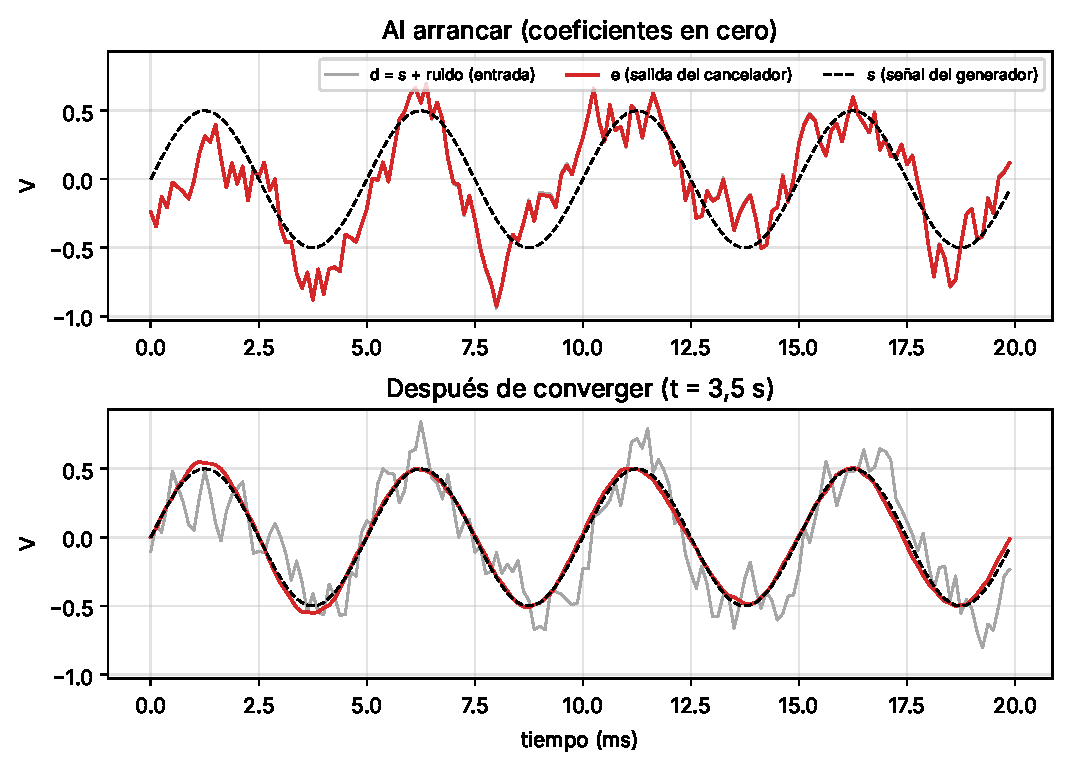
\includegraphics[width=0.9\linewidth]{p2_ondas.pdf}
\caption{Formas de onda (osciloscopio simulado) con $\mu = 0{,}005$: al arrancar la salida es
igual a la entrada ruidosa; a los 3,5~s el cancelador recupera la senoidal.}
\label{fig:ondas}
\end{figure}

\begin{figure}[H]
\centering
\begin{subfigure}{0.49\linewidth}
  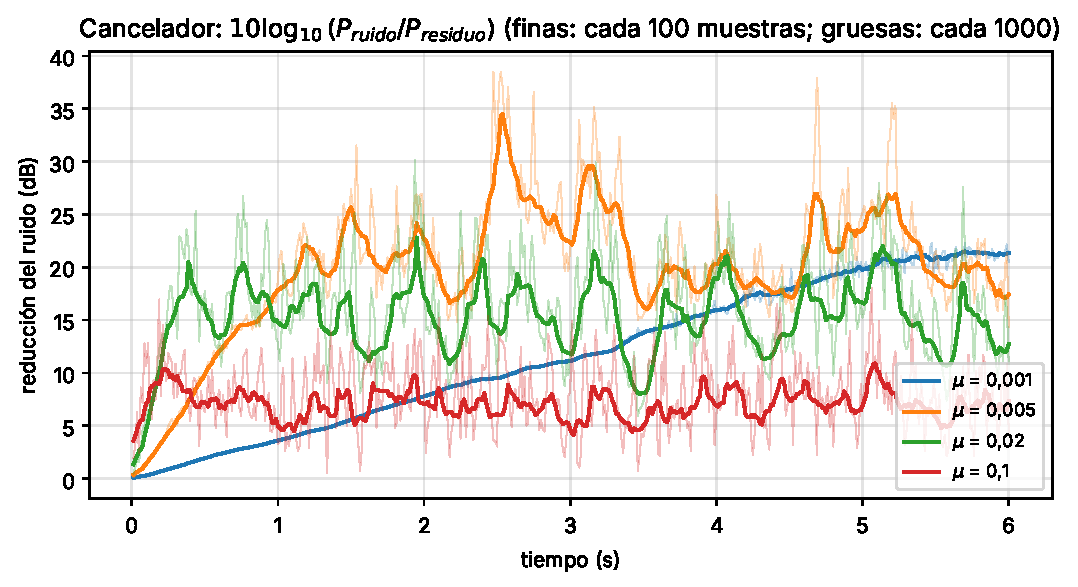
\includegraphics[width=\linewidth]{p2_e6_red.pdf}
\end{subfigure}
\begin{subfigure}{0.49\linewidth}
  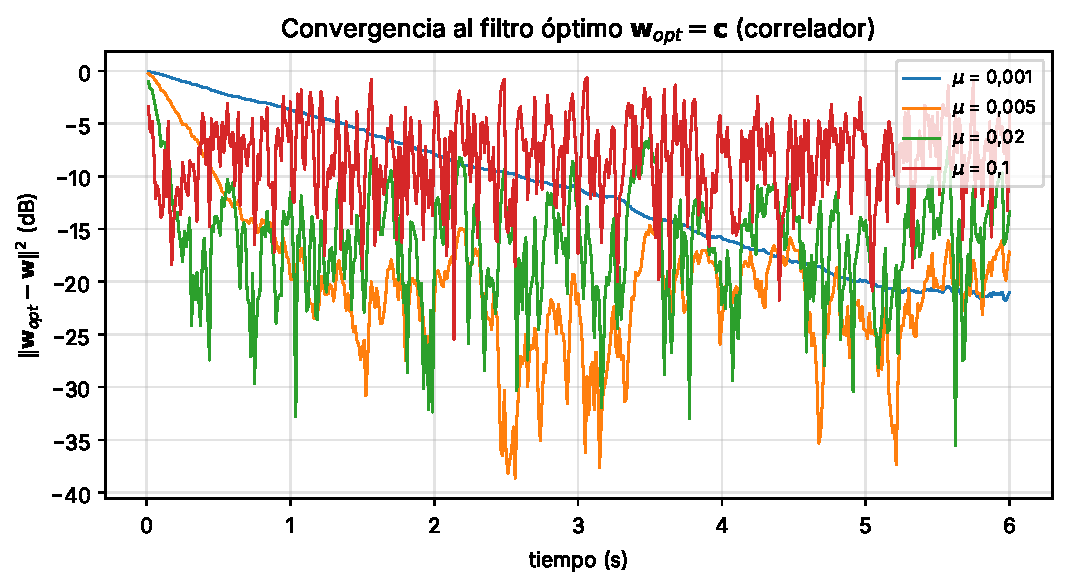
\includegraphics[width=\linewidth]{p2_e6_werr.pdf}
\end{subfigure}
\caption{Reducción de ruido y distancia al filtro óptimo $\mathbf{W}^* = \mathbf{c}$ para distintos $\mu$.}
\label{fig:e6}
\end{figure}

\begin{figure}[H]
\centering
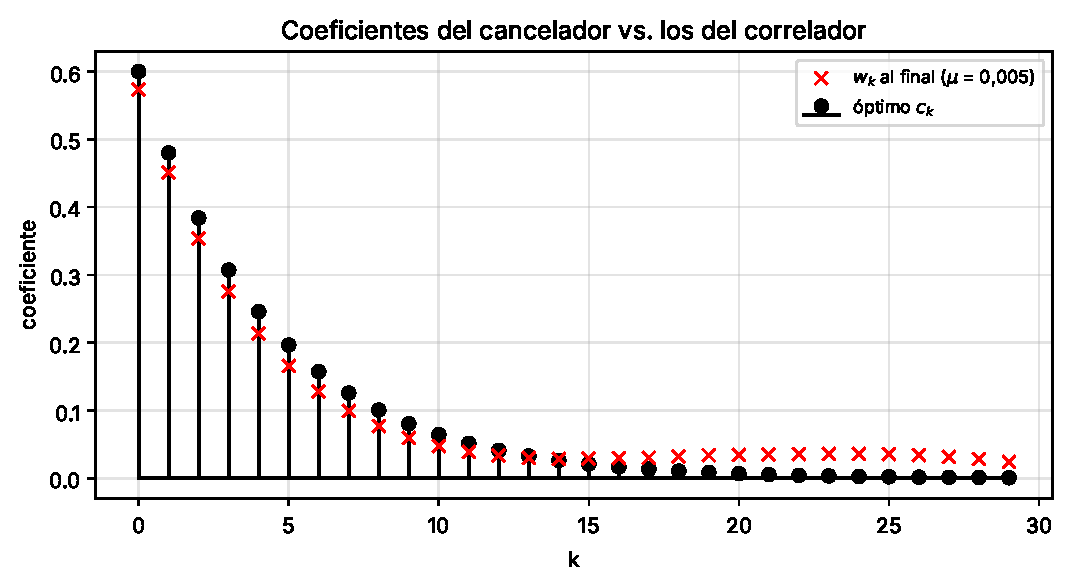
\includegraphics[width=0.8\linewidth]{p2_e6_coef.pdf}
\caption{Coeficientes del cancelador después de 6~s ($\mu = 0{,}005$): convergen al correlador.}
\label{fig:e6coef}
\end{figure}

\begin{itemize}
  \item El procesador converge al filtro óptimo de Wiener: los coeficientes copian al
  correlador (figura~\ref{fig:e6coef}) y $\|\mathbf{W}^*-\mathbf{w}\|^2$ cae 20~dB o más
  (figura~\ref{fig:e6}).
  \item Acá $\xi_{min} = P_s = 0{,}125$~V$^2$ no es cero: \textbf{la propia señal útil hace de
  ruido para el algoritmo}, porque $e = s + (n'-y)$ y el LMS adapta con todo $e$. Por eso el
  desajuste deja un ruido residual $\approx M\,P_s$ y aparece el compromiso velocidad--calidad:
  con $\mu = 0{,}1$ converge en decenas de milisegundos pero la reducción no pasa de 7--8~dB; con
  $\mu = 0{,}001$ tarda varios segundos pero supera los 20~dB (tabla~\ref{tab:cancelador}).
  \item Con el correlador en la rama de la referencia (figura~\ref{fig:ref}) el filtro también
  converge, a $C^{-1}$, pero mucho más lento. La referencia ahora es ruido coloreado, con
  densidad espectral $P_r|C(e^{j\omega})|^2$ que va de $9P_r$ (en $\omega = 0$) a $0{,}11P_r$
  (en $\omega=\pi$): la dispersión de autovalores $\lambda_{max}/\lambda_{min} \approx 81$ hace
  que los modos lentos tarden 81 veces más que los rápidos, que fijan el $\mu$ máximo.
\end{itemize}

\begin{figure}[H]
\centering
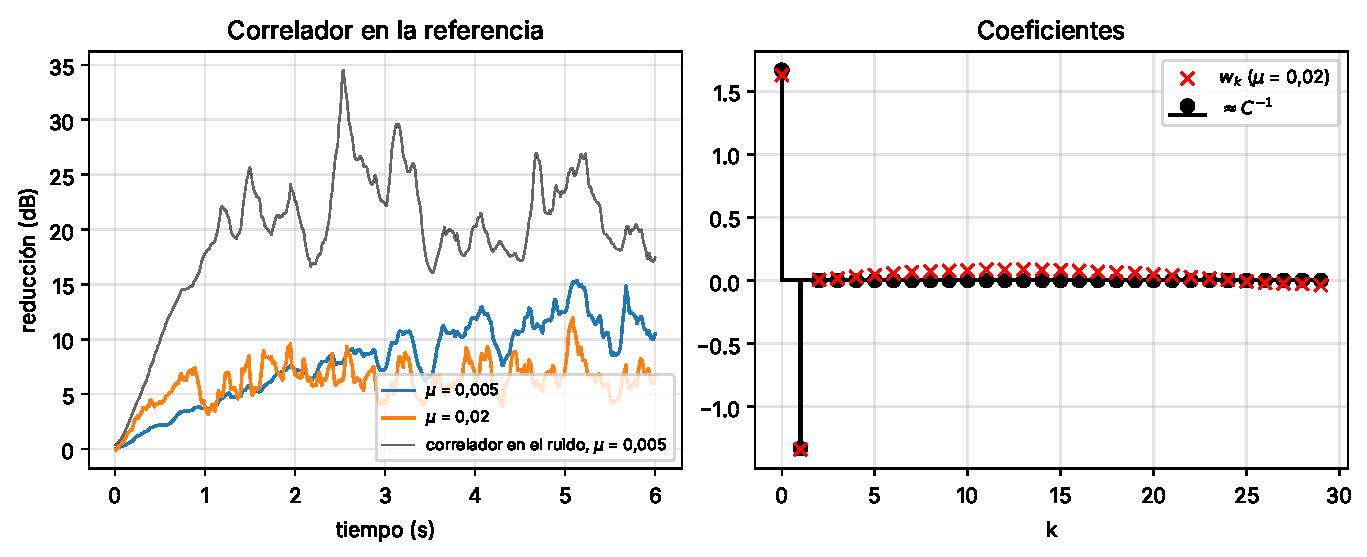
\includegraphics[width=\linewidth]{p2_e7_ref.pdf}
\caption{Correlador en la rama de la referencia (como en la figura 2 de la consigna).}
\label{fig:ref}
\end{figure}

\begin{table}[H]
\centering
\caption{Cancelador en régimen (simulación, promedio de los últimos 0,25~s de 6~s).}
\label{tab:cancelador}
\TablaCanceladorSim
\end{table}

\subsection{Resultados en la placa}
Para ver la convergencia en el osciloscopio: CH1 en la salida del DAC (J1-4) con la señal $e$
(comando \texttt{O1}), disparo externo en TRIG (J1-8), modo \emph{single}, y apretar SW2. Con
$\mu = 0{,}005$ ($\tau \approx 0{,}23$~s) se ve cómo la senoidal se va limpiando en el primer
segundo. Con \texttt{O0} se ve la señal con ruido y con \texttt{O4} el residuo.

\begin{figure}[H]
\centering
\begin{subfigure}{0.49\linewidth}\centering
  \figplaca[0.95\linewidth]{osc_d.png}{DAC = d (señal + ruido)}
  \caption{Entrada del cancelador, $d$.}
\end{subfigure}
\begin{subfigure}{0.49\linewidth}\centering
  \figplaca[0.95\linewidth]{osc_e.png}{DAC = e, ya convergido}
  \caption{Salida del cancelador, $e$.}
\end{subfigure}
\begin{subfigure}{0.98\linewidth}\centering
  \figplaca[0.8\linewidth]{osc_convergencia.png}{DAC = e, disparo en TRIG al apretar SW2, base de tiempo 100--200 ms/div}
  \caption{Aprendizaje después de reiniciar los coeficientes.}
\end{subfigure}
\caption{Capturas del osciloscopio.}
\end{figure}

\begin{figure}[H]
\centering
\figplaca{p2_e6_mu_red.png}{Reducción de ruido medida (tp4\_experimentos.m, sección E6)}
\caption{Reducción de ruido medida en la placa.}
\end{figure}

\paragraph{Tiempo de cómputo.} El comando \texttt{T} devuelve los ciclos promedio y máximo de la
interrupción completa (ruido, correlador, LMS y DAC). El pin PROC (J2-18) está en alto durante
ese tiempo, y en el osciloscopio se compara su ancho con el período de muestreo de 125~$\mu$s.
\completar{ciclos promedio y máximo de la línea P2T y ancho de PROC medido}

% ===========================================================================
\section{Conclusiones}
\begin{itemize}
  \item El LMS identifica una planta FIR de 30 coeficientes sin conocer nada de ella, sólo con su
  entrada y su salida. Con entrada aleatoria los coeficientes convergen exactamente a los de la
  planta, con la constante de tiempo que predice la teoría, $\tau = 1/(2\mu P_x)$.
  \item $\mu$ fija el compromiso central: más grande, más rápido, pero más ruido de gradiente
  (desajuste $M \approx \mu L P_x/2$) y, por encima de $2/(LP_x)$, divergencia. En la práctica
  el mejor $\mu$ está lejos del límite: cerca de él el aprendizaje es errático y más lento.
  \item La potencia de entrada cambia la escala de todo: con el LMS el mismo $\mu$ puede
  converger o diverger según la amplitud de la señal. El NLMS lo resuelve normalizando el paso, a
  costa de una división y de acumular la energía por muestra.
  \item La convergencia de los coeficientes requiere excitación: con entrada constante el MSE se
  anula pero sólo se aprende la ganancia de continua. Que el error sea chico no implica que el
  sistema esté identificado.
  \item En el cancelador el filtro converge al óptimo de Wiener, que es una copia del correlador,
  y recupera la senoidal. La señal útil actúa como ruido para el algoritmo, lo que obliga a usar
  $\mu$ chicos para lograr buena reducción. Cuando la referencia es coloreada, la dispersión de
  autovalores hace mucho más lenta la convergencia.
  \item Las tres implementaciones dan el mismo resultado; CMSIS-DSP es la recomendada en el
  Cortex-M por su costo en ciclos, y con 30 coeficientes el cancelador completo usa una fracción
  chica del período de muestreo.
\end{itemize}

% ===========================================================================
\clearpage
\appendix
\section{Código fuente}\label{sec:codigo}

El proyecto completo está en la carpeta \archivo{TP4/} del repositorio
\begin{center}\url{\Repo}\end{center}
El firmware en \archivo{TP4/source/}, los scripts de MATLAB en
\archivo{TP4/matlab/} y la simulación en la PC en \archivo{TP4/tools/host_sim/}.
Se listan los archivos principales.

\codigo{../../TP4/source/lms.h}{\archivo{lms.h}}
\codigo{../../TP4/source/lms.c}{\archivo{lms.c}}
\codigo{../../TP4/source/parte1.c}{\archivo{parte1.c}}
\codigo{../../TP4/source/parte2.c}{\archivo{parte2.c}}
\codigo{../../TP4/source/coefs.c}{\archivo{coefs.c}}
\codigo{../../TP4/source/fir_fijo.h}{\archivo{fir_fijo.h}}
\codigo{../../TP4/source/prng.h}{\archivo{prng.h}}
\codigo{../../TP4/source/main.c}{\archivo{main.c}}
\codigo{../../TP4/source/app_config.h}{\archivo{app_config.h}}
\codigo[language=Matlab]{../../TP4/matlab/tp4_captura.m}{\archivo{tp4_captura.m}}

\end{document}
